\documentclass{standalone}
\usepackage{newtx}
\usepackage{tikz-qtree}
\tikzset{edge from parent/.append style={semithick}} % thicker edges
\tikzset{every tree node/.style={align=center,anchor=north}}
\begin{document}
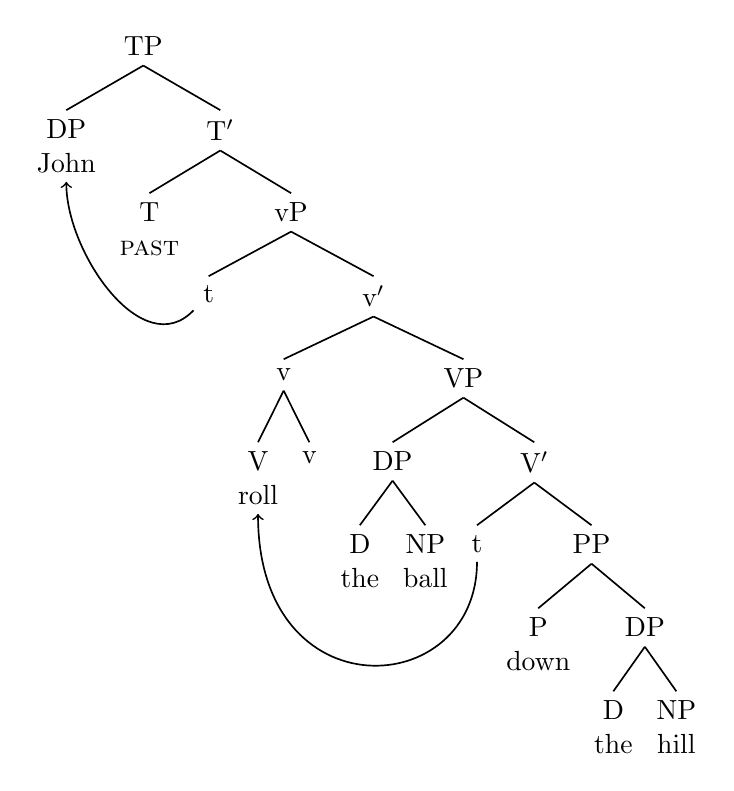
\begin{tikzpicture}
\Tree
[.TP
    [.\node(tgt1){DP\\John}; ]
    [.T$'$
        [.T\\\textsc{past} ]
        [.vP
            [.\node(src1){t}; ]
            [.v$'$
                [.v
                    [.\node(tgt2){V\\roll}; ]
                    [.v ] ]
                [.VP
                    [.DP
                        [.D\\the ]
                        [.NP\\ball ] ]
                    [.V$'$
                        [.\node(src2){t}; ]
                        [.PP
                            [.P\\down ]
                            [.DP
                                [.D\\the ]
                                [.NP\\hill ] ] ] ] ] ] ] ] ]
%\draw[semithick,->] (src1) .. controls +(south west:1) and +(south:2) .. (tgt1);
\draw[semithick,->] (src1) to[out=south west,in=south] (tgt1);
\draw[semithick,->] (src2) .. controls +(south:2) and +(south:3) .. (tgt2);
\end{tikzpicture}
\end{document}

